\subsection{Conclusion and advices}

\label{sec:results}

\begin{frame}{Implementation details}
	\vfill	
	\textbf{Deep Learning framework:} \texttt{Pytorch}. Easy to use (Python!), fast to learn (1h tutorial), a lot of already available architectures
	\vfill
	\textbf{Net architecture:} Alexnet. Begin with a little network (fast to train) to determinate the meta-parameters, then move to a deeper net (VGG).
	\vfill
	\textbf{Size of the training dataset:} 400 triplets (400 * 3 images * 2 modalities). Small dataset automatically created. I use \textbf{pre-trained network}!
	\vfill
\end{frame}

\begin{frame}{Trends: Robotics}

	Using deep learning as tools within classical framework:
	\begin{itemize}
		\item Improving monocular SLAM
		\item Global descriptor to find loop closure
	\end{itemize}
	\begin{figure}
		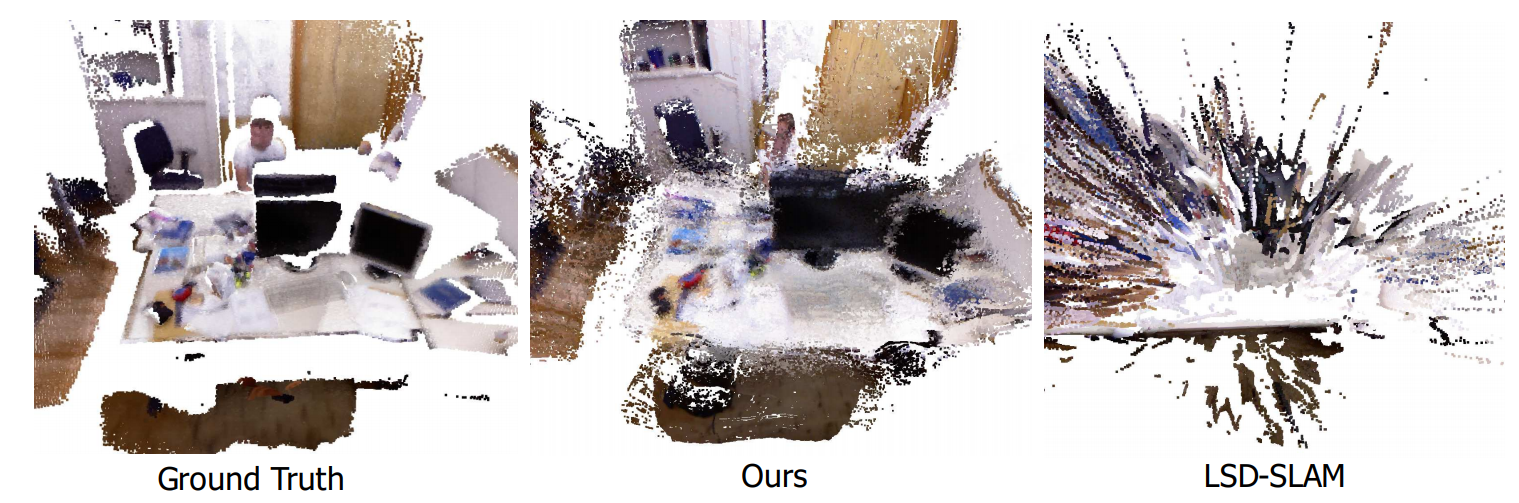
\includegraphics[width=0.9\linewidth]{images/cnnslam.png}
		\caption{Pure rotational camera motion SLAM problem solved, CNN-SLAM~\cite{POINTNET}}
	\end{figure}
	
\end{frame}

\begin{frame}{Trends: Computer Vision}

	Semi-supervised/unsupervised architecture:
	
	\begin{figure}
		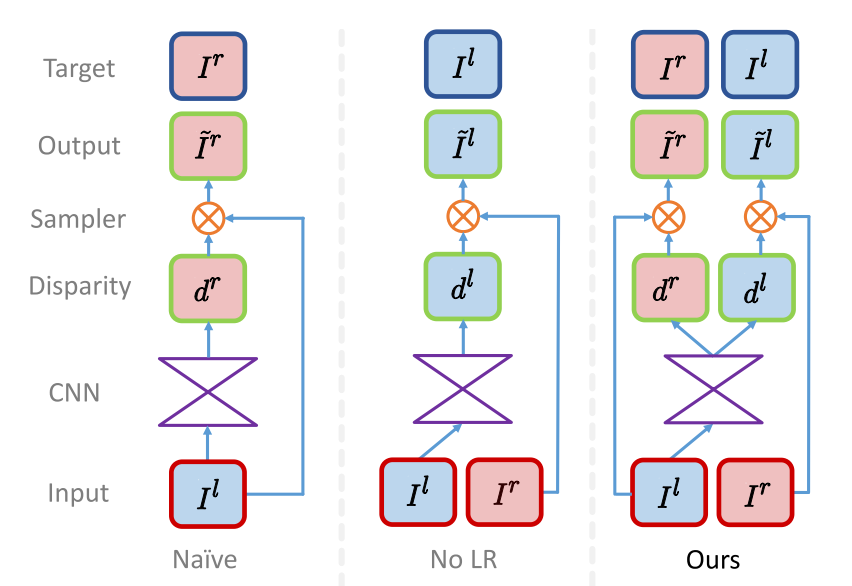
\includegraphics[width=0.7\linewidth]{images/unsupervised.png}
		\caption{Disparity from mono using stereo pairs as training data~\cite{UNSUPERVISED}}
	\end{figure}

\end{frame}

\begin{frame}{Trends: Computer Vision}

	Multi-task learning:
	
	\begin{figure}
		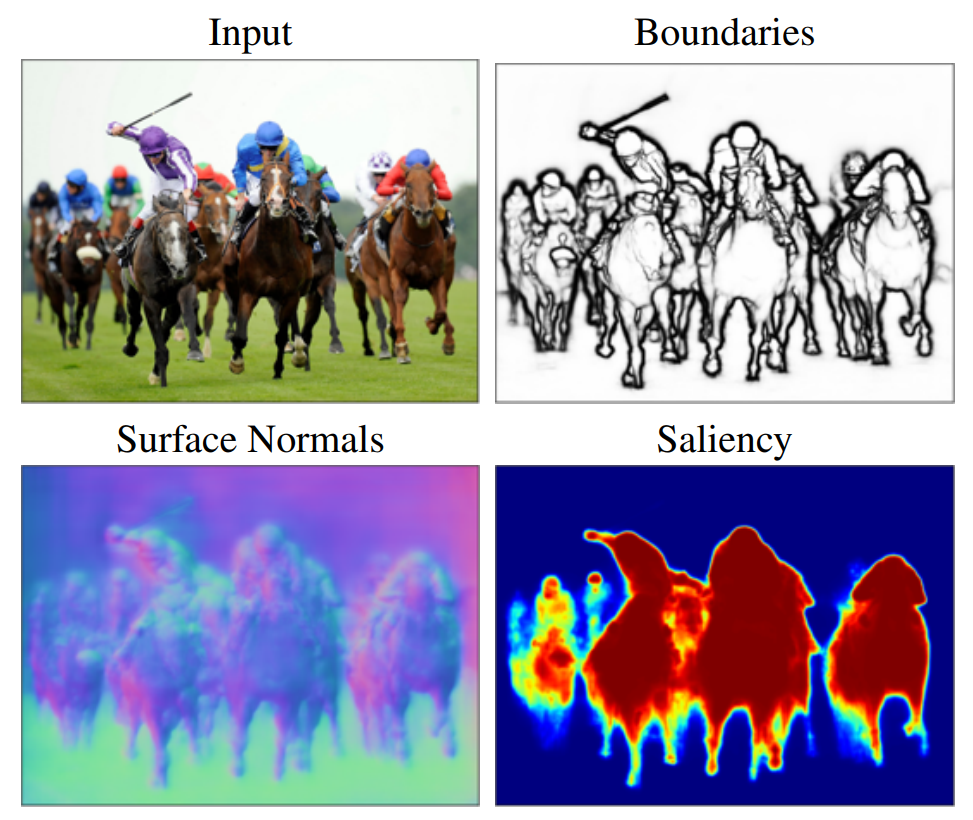
\includegraphics[width=0.45\linewidth]{images/ubernet1.png}
		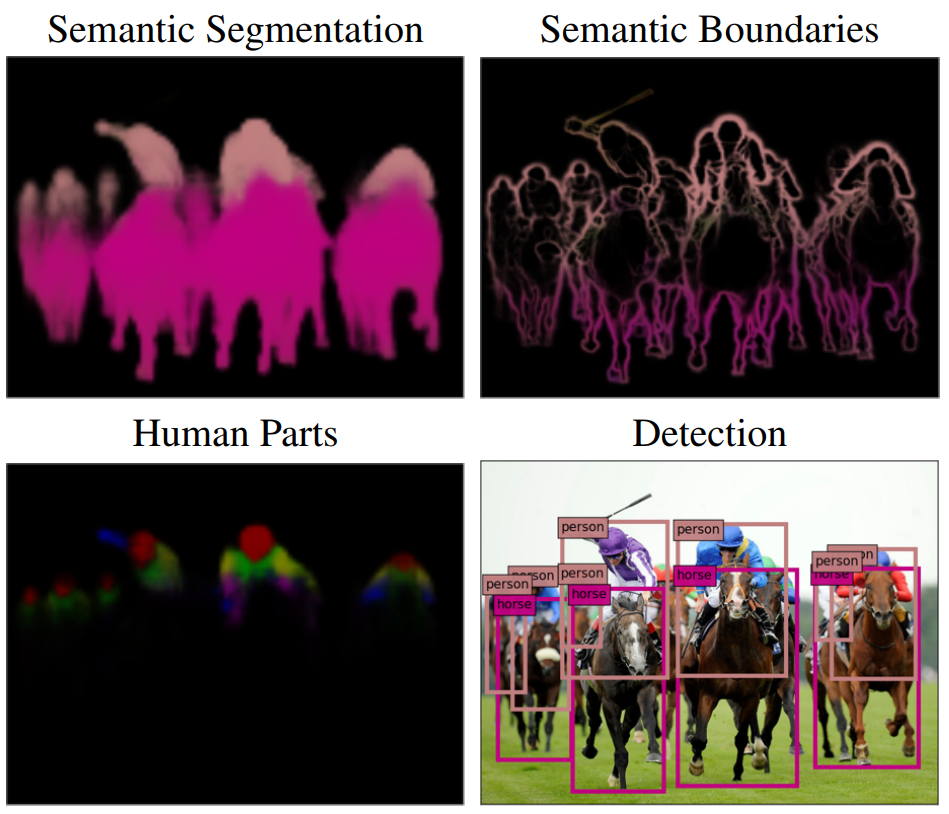
\includegraphics[width=0.44\linewidth]{images/ubernet2.png}
		\caption{Adding sub-goal increase accuracy over all tasks~\cite{UBERNET}}
	\end{figure}

	

\end{frame}

\begin{frame}{Trends: Computer Vision}

	No longer limited to RGB modality:
	\begin{itemize}
		\item Deep Learning on Points Cloud, Graph
		\item Modality fusion (RGB + Depth map)~\cite{FUSENET}
		\item Multi-spectral images (remote sensing field)
	\end{itemize}
	\begin{figure}
		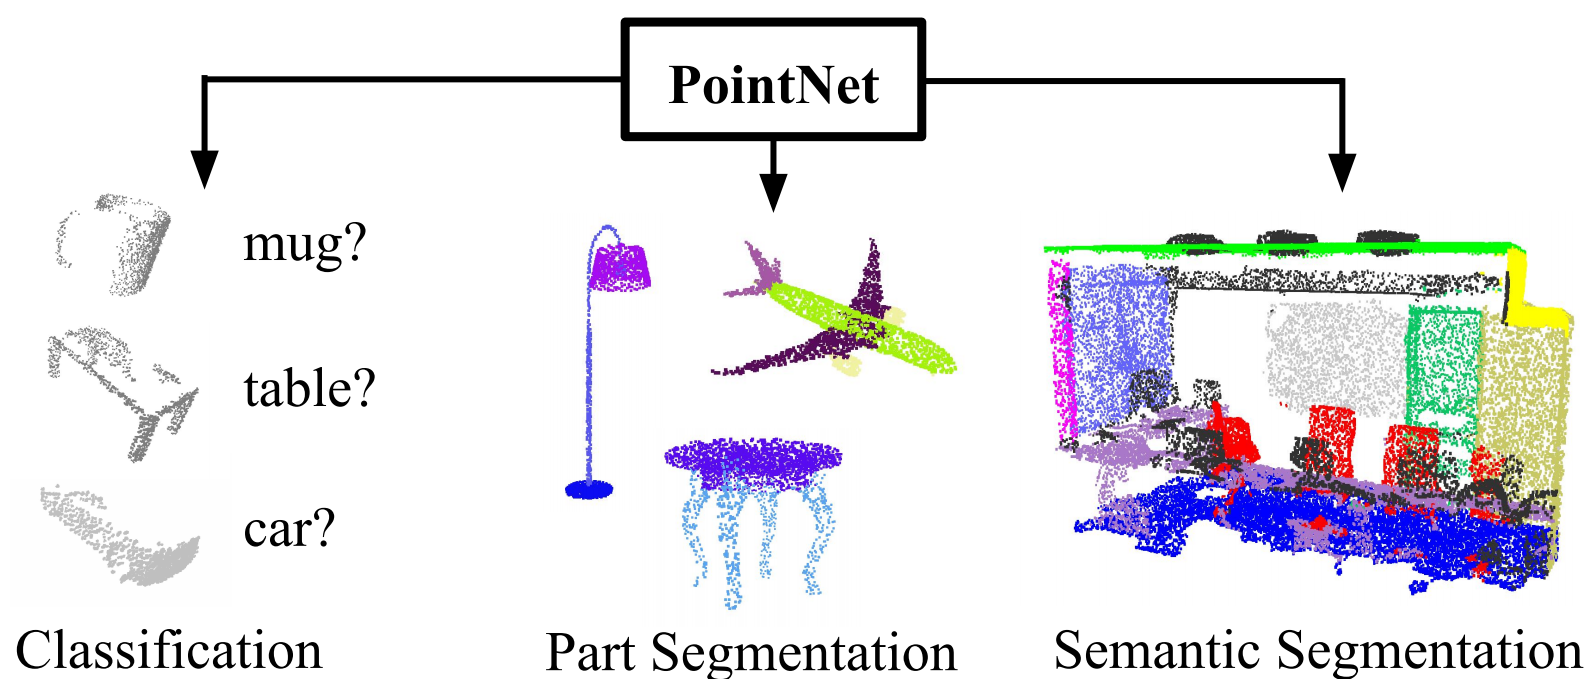
\includegraphics[width=0.6\linewidth]{images/pointnet.png}
		\caption{PointNet~\cite{POINTNET}}
	\end{figure}

\end{frame}